\documentclass[a4paper,10pt]{report}
\usepackage[utf8]{inputenc}
\usepackage{geometry}
\usepackage{graphicx}
\usepackage{tocbibind}
\usepackage[hidelinks]{hyperref}

% Title Page
\title{Development}
\author{Titouan FREVILLE}

\begin{document}
\maketitle
\tableofcontents
\listoffigures
\begin{abstract}
\end{abstract}

\part{Project global Organistation}
  \begin{figure}[h!]
    \centering
    \caption{\label{gpo} Global Project Organistation diagram}
    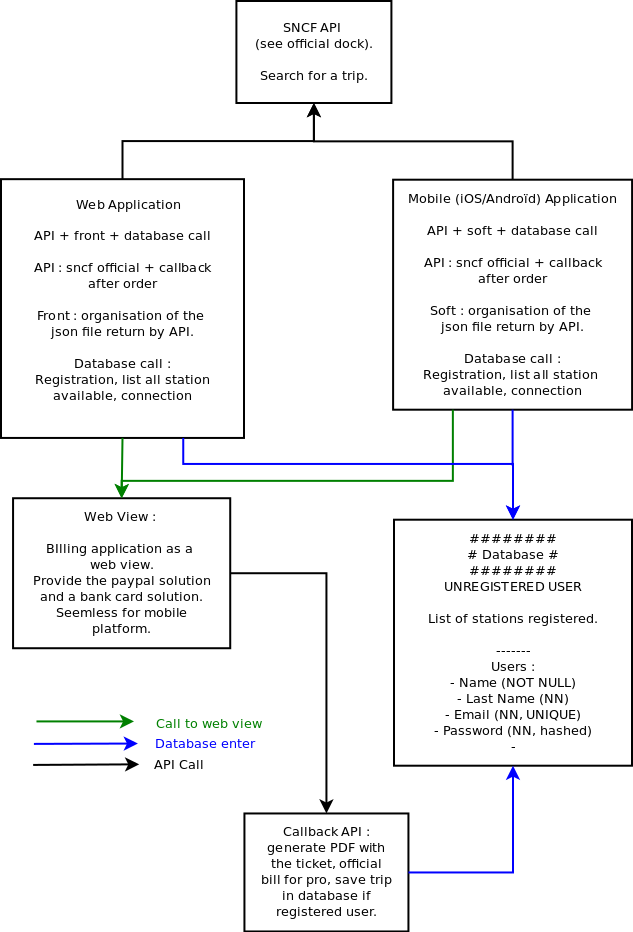
\includegraphics[scale=0.5]{./diagrams/gpo.png}
  \end{figure}
  The project will be build as describe as in the previous diagram. It use two 
apis, three applications and a database. The database will store registered 
users data and station available in as start and end point. The applications 
have the same functionalities (provide an interface for the user to search and 
select is trip), on three different devices (iOS, Androïd and web). Once the 
trip is selected, they will call the same web view to bill the client. The API 
will be use to acquire data from station (SNCF API) and generate PDF and bill. 
\href{https://data.sncf.com/api/fr/documentation}{For information on the SNCF 
API, please refer to the official 
documentation}(https://data.sncf.com/api/fr/documentation) 
\part{Callback API}
  This API will be done in Golang (or NodeJS if we run out of time). It will take the name of the client, the trip he choose, its price and a boolean
  for . Those informations
  will be used ot make the PDF tickets and a bill if needed.
\end{document}          
